% Speaker notes for slides/workshop.tex.
% Build from the repository root:   make speaker-notes
% (equivalently: cd slides && tectonic --keep-intermediates workshop.tex && tectonic speaker-notes.tex)
% Notes flow continuously; each entry shows one slide in its final click state. The slide-to-page map is read from
% workshop.nav, so the notes stay aligned when overlays change. If frames are added or
% removed, renumber the \snote calls below.
\documentclass[11pt]{article}
\usepackage[a4paper,margin=14mm,top=12mm,bottom=16mm]{geometry}
\usepackage{amsmath,amssymb,graphicx,xcolor,enumitem,booktabs,array,microtype}
\usepackage[hidelinks]{hyperref}
\definecolor{ink}{HTML}{171717}
\definecolor{accent}{HTML}{4E5AFF}
\definecolor{danger}{HTML}{B53248}
\definecolor{paper}{HTML}{F4F6FC}
\renewcommand{\familydefault}{\sfdefault}
\setlength{\parindent}{0pt}
\setlength{\parskip}{5pt}
\pagestyle{plain}
\setlist{nosep,leftmargin=1.2em}
\newcommand{\F}{\mathbb F}

% ---------------------------------------------------------------- slide -> page map
\makeatletter
\newcount\tfc@n
\def\headcommand#1{#1}
\def\beamer@framepages#1#2{\global\advance\tfc@n by 1
  \expandafter\xdef\csname tfc@first@\the\tfc@n\endcsname{#1}%
  \expandafter\xdef\csname tfc@last@\the\tfc@n\endcsname{#2}}
\def\partentry#1#2{}
\def\sectionentry#1#2#3#4#5{}
\def\beamer@subsectionentry#1#2#3#4#5{}
\def\slideentry#1#2#3#4#5#6{}
\def\beamer@partpages#1#2{}
\def\beamer@sectionpages#1#2{}
\def\beamer@subsectionpages#1#2{}
\def\beamer@documentpages#1{}
\def\beamer@appendixpages#1{}
\def\translate#1{}
\IfFileExists{workshop.nav}{\input{workshop.nav}}{%
  \PackageError{speaker-notes}{workshop.nav not found}{Run: tectonic --keep-intermediates workshop.tex}}
\newcommand{\firstpage}[1]{\csname tfc@first@#1\endcsname}
\newcommand{\lastpage}[1]{\csname tfc@last@#1\endcsname}
\makeatother

% ---------------------------------------------------------------- continuous layout
\def\pendingtransition{}
\newcommand{\transition}[2]{\gdef\pendingtransition{%
  {\color{accent}\rule{\linewidth}{0.9pt}}\par\vspace{-3pt}
  {\bfseries\color{accent}Slide #1, section title.}\enspace{\small #2}\par\vspace{6pt}}}
\newcommand{\snote}[6]{%
  \par\medskip\noindent
  \begin{minipage}{\linewidth}
    \pendingtransition\gdef\pendingtransition{}%
    {\large\bfseries\color{accent}#1\enspace}{\large\bfseries #2}\hfill
    {\footnotesize start \textbf{#3}\quad clicks \textbf{\the\numexpr\lastpage{#1}-\firstpage{#1}\relax}\quad
     pdf page \lastpage{#1}}\par
    \vspace{-4pt}{\color{gray!45}\rule{\linewidth}{0.4pt}}\par\vspace{3pt}
    \begin{minipage}[t]{0.36\linewidth}\vspace{0pt}
      \fcolorbox{gray!55}{white}{\includegraphics[page=\lastpage{#1},
        width=\dimexpr\linewidth-2\fboxsep-2\fboxrule\relax]{workshop.pdf}}
    \end{minipage}\hfill
    \begin{minipage}[t]{0.61\linewidth}\vspace{0pt}
      \setlength{\parskip}{4pt}#4
    \end{minipage}
  \end{minipage}\par
  {\small\setlength{\parskip}{3pt}%
   \if\relax\detokenize{#5}\relax\else\textbf{\color{accent}Do.}\enspace #5\par\fi
   \if\relax\detokenize{#6}\relax\else\textbf{\color{danger}If asked.}\enspace #6\par\fi}}

\begin{document}

% ================================================================ cover
{\LARGE\bfseries Training for Constraining: speaker notes\par}
\vspace{2pt}
{\normalsize Levi Katyal Sledd and Vijay Singh \quad$\cdot$\quad Devcon~8 workshop \quad$\cdot$\quad
notes for \texttt{slides/workshop.pdf} as of 28 October 2026\par}
{\color{accent}\rule{\linewidth}{0.7pt}}

\textbf{How to read.} The notes run continuously in slide order. Each entry shows the slide in its
final click state beside the talking track (\textbf{Say}), followed by stage directions (\textbf{Do})
and backup answers or cautions (\textbf{If asked}). \emph{Clicks} counts the advances inside a slide;
\emph{start} is minutes into a 50-minute run. Section-title slides appear as headings.

\textbf{Core message.} A proof system can be perfectly sound while the application is broken, because
the proof is about the constraints that were written, not the relation that was meant.

\textbf{Timing plan} (a proposal; calibrate in rehearsal)\par\vspace{2pt}
{\small
\begin{tabular}{@{}lllll@{}}\toprule
Section & Slides & Start & Length & Who\\\midrule
Opening and motivation & 1--4 & 0:00 & 3:30 & \\
Circuits and constraints & 5--12 & 3:30 & 8:45 & \\
Patterns, Example 0, Example 1 & 13--21 & 12:15 & 7:45 & \\
Exercise 2 (selector, pairs) & 22--24 & 20:00 & 5:00 & \\
Example 3 (range, foreign field) & 25--30 & 25:00 & 6:15 & \\
Deep dive: gnark fake GLV & 31--37 & 31:15 & 7:00 & \\
Finding underconstraints, demo & 38--43 & 38:15 & 6:00 & \\
Verification infrastructure, AI & 44--47 & 44:15 & 3:15 & \\
Wrap-up and questions & 48--49 & 47:30 & 2:30 & \\\bottomrule
\end{tabular}\par}
The two \verb|\note| timings inside \texttt{workshop.tex} (slides 12 and 14) predate Levi's revision and
are superseded by this plan. \textbf{If behind schedule,} compress slides 9, 27 and 29 to one sentence
each, and protect the exercise (23--24), the fake-GLV arc (32--37), the demo (42) and the close (49).

\textbf{Before presenting}
\begin{enumerate}[leftmargin=1.4em,itemsep=2pt]
\item \textbf{Make the repository public.} The QR codes on slides 1 and 49 point to the repository,
  which returns 404 to the audience while it is private.
\item \textbf{Confirm the slot length.} The title slide says 50 minutes; Devcon~8 lists workshops at 60.
  With 60, give the extra time to the exercise and to questions.
\item \textbf{Remove drafting text printed on slides.} Slide 35 (``supplied HTML case study''), slide 37
  (``verify precise affected paths and releases''), slide 51 (``Supplied reference:
  fake-glv-underconstraint.html'' and ``Check the release advisory''). Replacement facts, checked against
  gnark's source, are in the notes for slides 35 and 37.
\item \textbf{Slide 4, Airbender row.} A comment in the source questions whether these findings are
  circuit underconstraints. Verify against the report or drop the row.
\item \textbf{Preflight the demo on the presenting laptop}, offline: \texttt{make all} and \texttt{make lean}
  from the repository root, with a large terminal font.
\item \textbf{Slide 7} has an empty final click; click through it.
\item \textbf{Commit} \texttt{notes/smt-ring-theory.pdf} if you mention it on slide 43.
\end{enumerate}

\textbf{Closing line} (slide 49): \emph{A prover can replace every private witness and every hint. Only
enforced constraints bind the public claim. Check the assumptions of your dependencies and compilers,
not only your own code.}

% ================================================================ slides
\snote{1}{Title}{0:00}{%
Welcome. One sentence each to introduce yourselves; this is a hands-on session, so keep it short.

The claim for the next fifty minutes: a SNARK can be perfectly sound and the application still
broken, because the proof is about the constraints you wrote, not the relation you meant.

Plan: four small examples you can check by hand, one real bug in a widely used library, and the
tools that find these bugs.
}{%
Point at the QR code: everything we run today is in this repository and needs only Python~3.10.
Pause a few seconds for phones.
}{}

\snote{2}{Outline}{0:40}{%
One thread runs through every section: write the intended relation, build an adversarial witness,
watch the constraints accept it, repair, then ask how you would have found it.

Two interactive moments: a two-minute pair exercise in the middle and a live demo near the end.
}{Do not read the list aloud.}{}

\transition{3}{\emph{Motivation.} One breath, then advance.}
\snote{4}{Motivation: Underconstrained Circuits in 2026}{1:00}{%
Read the middle column, not the first. Every row is a property somebody assumed and nobody enforced.

Pick one row and tell it properly. Orchard: an elliptic-curve base-point cell was not bound, and the
reported consequence was counterfeit Orchard value. Then name the shape of the others: OpenVM did not
check that a hint lay in the right subfield; Scroll did not check G2 subgroup membership.

Mature, audited systems, all this year, the same shape. Then the caveat on the slide: discovery does
not establish prior exploitation.
}{%
Before the talk: verify or drop the Airbender row (see the cover page).
}{%
Sources for every row are on appendix slide 50. The rows have different consequences; do not say all
four were exploitable soundness failures. The slide's own footnote: Airbender was one critical
circuit bug and two verifier-composition flaws.
}

\transition{5}{\emph{Circuits and Constraints.} Say: ten minutes of shared vocabulary, so every later
example is precise. This is where the notation comes from.}
\snote{6}{Finite Fields}{3:30}{%
Every value in a circuit is an element of a finite field. Our running toy is $\F_{11}$.

$3\cdot7=21\equiv10$. You may reduce whenever you like, so $10=-1$. Division exists:
$3\cdot4=12\equiv1$, so $\tfrac13=4$.

Two facts will matter later, so say them now:
\begin{itemize}
\item a field has no zero divisors: $ab=0$ forces $a=0$ or $b=0$;
\item an equation in $\F_p$ is not an equation over the integers, because the field wraps around.
\end{itemize}
}{Four clicks. Keep moving; do not teach the definition of a field.}{%
``Why 11?'' Small enough to compute by hand. Every argument today either works over any field, or we
say explicitly that it does not.
}

\snote{7}{Relations and Witnesses}{4:30}{%
A zero-knowledge statement says: I know something secret that relates to something public.

Simple claim: I know $w$ with $x=w^4+5$. Here $w$ is the secret witness, $x$ the public witness,
and the relation $R(w,x)$ is the property we actually care about.

Everything else today is one question: does the circuit really enforce $R$?
}{The last click reveals nothing (a stray pause in the source). Click through it.}{}

\snote{8}{Relations and Witnesses: Merkle Example}{5:30}{%
In practice both witnesses are vectors, and the public part can be inputs, outputs, or both.

Real example: four secret leaves and one public root. The relation says the leaves hash up to the
root, $H(H(w_0,w_1),H(w_2,w_3))=x_0$. Red is public, blue is secret; the deck keeps that colour
convention.

Keep this picture in mind. If a circuit computes a root but never constrains it to equal the public
$x_0$, the proof says nothing about these leaves. That is Example~0.
}{The tree appears on the third click. Point at the root, then the leaves.}{%
``A Merkle proof is one leaf plus a path.'' Yes; the slide shows the whole tree for simplicity. The
authentication-path version has the same public and secret split.
}

\snote{9}{Arithmetic Circuits and Constraints}{7:00}{%
An arithmetic circuit is a Boolean circuit whose wires carry field elements and whose gates are
$+$ and $\cdot$.

Each gate becomes a polynomial equation, so from here on ``circuit'' and ``constraint system'' mean
the same thing: a system of polynomial equations, and only those equations are enforced.
}{}{%
``Is it really one constraint per gate?'' Not literally. R1CS, PLONKish and AIR package gates
differently. The point that survives is that the circuit is a set of polynomial equations.
}

\snote{10}{Example: Constraint System and Witnesses}{7:45}{%
Four constraints compute $w_0^4+5$: square twice, add five. $C_3$ ties the result to the public
$x_0$.

Vocabulary, one click each: $x$ is public; $w=(w_0)$ is secret; $w_1,w_2,w_3$ are intermediate
witnesses, also secret; $\overline w$ is the extended witness, everything the prover fills in;
$(\overline w,x)\vDash C$ means every constraint holds.

Last line: for this system, satisfying $C$ is exactly the relation. Remember $C_3$. In five minutes
we delete it.
}{%
Five clicks. Where the last line writes $(w,x)\vDash C$, say ``the extended witness satisfies $C$''.
}{}

\snote{11}{A SNARK Only Proves the Encoded Relation}{9:30}{%
The pipeline: an intended specification $R$ is encoded as constraints $C$; the prover produces a
proof; the verifier checks it.

The proof system guarantees one thing: the prover knows an extended witness satisfying $C$. It knows
nothing about $R$.

Ideally the two agree in both directions. Left to right is soundness of the circuit: everything
accepted is true. Right to left is completeness: every true statement can be proven. Underconstrained
means left to right fails, and that is today's topic. The footnote is the weaker, public-statement
version with existential quantifiers.
}{Gesture at the ``encode'' arrow: every bug today lives on that arrow.}{%
``What about overconstrained?'' That breaks completeness: honest provers get stuck. Annoying, not
exploitable, which is why we focus on soundness.
}

\snote{12}{Hints}{11:00}{%
Some values are expensive or impossible to compute with $+$ and $\cdot$, such as inverses or bit
decompositions. The prover computes them outside the circuit. That is a hint; the honest witness
generator's answer is called advice.

Left: the honest computation $t\leftarrow w^2$. Right: what is enforced, $t-w^2=0$.

The blue box is the most important sentence today: the prover may replace the witness generator.
Anything not constrained is chosen by the attacker.

A hint is not unsafe by itself. It needs enough constraints to establish the property the rest of
the circuit relies on, not necessarily a unique value. Slide 21 makes that precise.
}{}{}

\transition{13}{\emph{Kinds of Underconstraint Bugs.} Say: four worked examples, each one row of the
next table.}
\snote{14}{Common Failure Patterns}{12:15}{%
Five missing requirements:
\begin{itemize}
\item copy constraints: wires that should agree do not;
\item range checks: field elements have no order, so ``small'' must be enforced;
\item hint validation: the prover controls a computation;
\item field or group membership: an identity holds, but in a bigger domain than intended;
\item public binding: inputs or outputs float free of the circuit.
\end{itemize}
Roadmap: Example~0 is public binding, Example~1 hint validation, Exercise~2 and Example~3 range
checks, and fake GLV combines a range problem with group membership. Mention disabled selectors and
branch coverage. The categories overlap.
}{One minute. It is a map, not a lecture.}{}

\transition{15}{\emph{Example 0: Missing Public Output Binding.}}
\snote{16}{Example: Missing Copy Constraint/Public Binding}{13:15}{%
Take the constraint system from slide 10 and delete $C_3$.

Ask the room: after the deletion, which constraint mentions $x_0$? None.

The private computation is still internally consistent; it computes $w_0^4+5$ into $w_3$. Nothing
connects it to the public value, so for every $x_0$ any $w_0$ works.
}{Ask the question and wait two seconds before answering.}{}

\snote{17}{Example 0: Missing Binding $\to$ False Proof}{14:15}{%
A concrete false claim: I know $w_0$ with $7=w_0^4+5$, so $w_0^4=2$.

The table lists every fourth power in $\F_{11}$: only $0,1,3,4,5,9$. Two is not there, so no honest
witness exists and the statement is false.

Yet $\overline w=(1,1,1,6)$ with $x_0=7$ satisfies all three remaining constraints. That is a valid
proof of a false statement, with the proof system working perfectly.
}{This is the ``missing public binding'' line of \texttt{make demo}.}{%
``Why so few fourth powers?'' $\F_{11}^\times$ is cyclic of order 10 and $\gcd(4,10)=2$, so
$w\mapsto w^4$ reaches only five nonzero values.
}

\snote{18}{Repair: Public Input Binding}{16:00}{%
Put the copy constraint back. Now satisfying the constraints is equivalent to the relation.

That single equation is the only link between what the circuit computes and what the verifier sees.
In the Merkle picture it is the constraint that the computed root equals the public root.
}{The title says ``Input''. Say ``public output binding'', matching the section.}{}

\transition{19}{\emph{Example 1: Unvalidated Hints.}}
\snote{20}{Example 1: An Unvalidated IsZero Hint}{17:00}{%
IsZero is everywhere: comparisons, conditionals, ``is this balance empty''.

Secret $w$, public output $x$, relation $x=\operatorname{IsZero}(w)$. IsZero cannot be computed with
$+$ and $\cdot$ alone, so a hint helps: $h=w^{-1}$ when $w\ne0$, otherwise $0$. The only constraint is
$x=1-wh$.

Honest prover: works. Attacker: take $w=3$ and set $h=0$. Then $x=1$, a proof that
$\operatorname{IsZero}(3)=1$. The honest generator never outputs $h=0$ for nonzero $w$, but the
attacker does not run the honest generator.
}{}{%
``But $w$ is secret, and $x=1$ is honest for $w=0$.'' True for the gadget in isolation. In a real
circuit $w$ is a wire constrained elsewhere, such as a committed balance, and the gadget lets the
prover output the wrong bit for that particular $w$. Soundness is per witness (slide 11).

General attack: for any nonzero $w$ and any target $x$, set $h=(1-x)w^{-1}$.
}

\snote{21}{Repair: Constrain the Hint's Effect}{18:45}{%
Add $wx=0$.

If $w\ne0$, no zero divisors force $x=0$, and then $x=1-wh$ forces $h=w^{-1}$.

If $w=0$, the first constraint forces $x=1$ and $h$ can be anything. That is fine: a free hint is
harmless when it cannot reach the public output. Witness non-uniqueness is not underconstraint.

The lesson box: pin down public behaviour, not internal encodings.
}{}{%
``Isn't a free $h$ a bug?'' Over $\F_{11}$ the repaired constraints accept exactly 21 triples
$(w,h,x)$, and all 21 have the correct $x$; $h$ is free only when $w=0$. Determinism checkers such as
Picus ask whether outputs are determined by inputs, and a free $h$ does not violate that.
}

\transition{22}{\emph{Exercise 2: A Selector.} Ask people to find a neighbour.}
\snote{23}{Exercise 2: A Selector}{20:00}{%
Intended behaviour: $s$ selects $x$ or $y$. Implemented: one equation, $z=sx+(1-s)y$.

Here $x$, $y$ and $s$ are secret and $z=5$ is public. With $x=3$ and $y=7$: can you find an $s$ that
makes the equation accept? Which constraint is missing?

Two minutes with your neighbour.
}{%
Start a visible two-minute timer. Do not advance until someone has answered. If the room is stuck,
hint: solve the equation for $s$.
}{%
Answer key: $s=\dfrac{z-y}{x-y}=\dfrac{-2}{-4}=\dfrac12=6$ in $\F_{11}$.
}

\snote{24}{Selector: False Witness and Repair}{23:00}{%
$s=6$: $6\cdot3+(1-6)\cdot7=18-35=-17\equiv5$, and 5 is neither input.

A nice way to see it: 6 is $\tfrac12$ in $\F_{11}$, and 5 is the midpoint of 3 and 7. The equation is
linear interpolation; it accepts every point on the line through $x$ and $y$.

Repair: $s(s-1)=0$. No zero divisors, so $s\in\{0,1\}$ and the output is $x$ or $y$. The argument
uses nothing about 11: it holds in every field, and the repository has it as a machine-checked Lean
theorem, \texttt{selector\_sound}.
}{%
Optional: show the ``non-Boolean selector'' line of \texttt{make demo}, or open
\nolinkurl{lean/Workshop/Selector.lean}.
}{%
``Why every field?'' Only the zero-product rule is used. In $\mathbb Z/6$, $s=3$ satisfies
$s(s-1)=0$ and breaks the selector. For ``but $x,y$ are secret'', give the IsZero answer (slide 20).
}

\transition{25}{\emph{Example 3: Range Checks and Foreign-Field Arithmetic.} Say: this is the bridge
to the gnark case study.}
\snote{26}{A Boolean Check Is a 1-Bit Range Check}{25:00}{%
$s(s-1)=0$ is a range check on a single bit.

Fields have no order and no sign: in $\F_{11}$, $3-5=9$. So any claim like
``balance $\ge$ withdrawal'' needs an explicit range check: read the value as an integer in
$\{0,\dots,p-1\}$ and prove it is below $2^n$.
}{}{}

\snote{27}{Range Checks by Bit Decomposition}{26:00}{%
To show $x<4$: two Boolean bits and $x=w_0+2w_1$, so $x\in\{0,1,2,3\}$.

Pitfall: this needs $2^n\le p$. With four bits in $\F_{11}$, $3=1+2$ and also $3=2+4+8-11$: two bit
patterns for the same $x$. A circuit that reads the top bit as ``$x\ge8$'' lets the prover claim
$3\ge8$.

This is circomlib's Num2Bits pattern. A CAV 2024 crawl found bitsums in 98\% of public Circom
projects. It is also the pattern that made SMT solvers time out; we come back to that on slide 43.
}{If behind schedule, give only the pitfall sentence.}{}

\snote{28}{Foreign-Field Arithmetic}{27:30}{%
Sometimes the circuit lives in $\F_p$ but must check arithmetic modulo a different number $\ell$.
Elliptic-curve scalars are the standard case.

Toy: native $\F_{11}$, foreign modulus 3, public $x,y,z\in\{0,1,2\}$ already range-checked. We want
$xy\equiv z\pmod3$, that is $xy-z=3k$ over the integers.

The prover supplies the quotient $k$ as a hint $w$; we constrain $xy-z=3w$ and $w$ Boolean. Example:
$2\cdot2=4\equiv1$, quotient 1.
}{}{}

\snote{29}{Range-Check for Sound Modular Arithmetic}{28:45}{%
Why is this sound? The equation holds in $\F_{11}$, so $xy-z-3w$ is a multiple of 11 as an integer.

With the ranges, that integer lies in $\{-5,\dots,4\}$, and the only multiple of 11 there is 0. So the
equation holds over the integers, and the congruence mod 3 follows.

The range checks are what let you lift a field equation to an integer equation. Remember this
argument: it is exactly what the gnark repair needs, and it is the kind of reasoning SMT solvers find
hardest.
}{If behind schedule, give only the last paragraph.}{%
``Does a Boolean quotient suffice for real curve arithmetic?'' No. Real gadgets use limbs and carries
with bounds on every term; a Boolean quotient works here only because the numbers are tiny.
}

\snote{30}{An Unbounded Quotient Checks Nothing}{30:00}{%
Now drop the Boolean constraint on $w$. Since 3 is invertible in $\F_{11}$,
$w=(xy-z)\cdot3^{-1}=(xy-z)\cdot4$ satisfies the equation for any $x,y,z$.

False claim: $2\cdot2\equiv0\pmod3$. Take $w=5$: $3\cdot5=15=4$ in $\F_{11}$, so it passes. Over the
integers $4=15$ is false; the field wrapped around.

Moral: the quotient and every other term must be range-checked.

Transition: now the same bug inside a widely used library.
}{This is the ``unbounded foreign-field quotient'' line of \texttt{make demo}.}{}

\transition{31}{\emph{Deep Dive: gnark Fake GLV.} Say: everything we need is already on the board:
two fields, a quotient, and a cancellation.}
\snote{32}{Fake GLV: Checking a Hinted Scalar Multiplication}{31:15}{%
Goal: prove $Q=[s]P$ cheaply. Instead of computing $[s]P$ in the circuit, the prover supplies $Q$ and
two short scalars $u,v$. The circuit checks a curve relation $[u]P=[v]Q$ and a scalar relation
$u\equiv sv\pmod\ell$. Short scalars roughly halve the cost of the curve check.

Correctness: substitute to get $[v](Q-[s]P)=O$, then cancel $v$. Cancelling needs two hypotheses:
$P,Q$ in the prime-order subgroup, and $v\not\equiv0\pmod\ell$.

``Every hypothesis needs enforcement'' is the checklist for the next five slides.
}{}{%
``Why are the scalars short?'' Appendix slide 53: lattice reduction outside the circuit gives
$|u|,|v|\approx\sqrt\ell$.
}

\snote{33}{Two Fields Meet in One Gadget}{32:30}{%
Two moduli. $r$ is the native field of the circuit, where curve coordinates live. $\ell$ is the
subgroup order, where scalars live.

For BabyJubjub inside a BN254 circuit, coordinates are native but $\ell\ne r$. So
$u\equiv sv\pmod\ell$ is foreign-field arithmetic: slide 28 with $\ell$ in place of 3. An equation
in $\F_r$ does not enforce it.
}{}{%
Do not conflate coordinate arithmetic, which is native here, with scalar arithmetic, which is
foreign.
}

\snote{34}{A Free Quotient Makes the Check Vacuous}{33:30}{%
The vulnerable pattern checks $u-sv=k\ell$ in $\F_r$, with $k$ a prover-supplied hint and no bound
on it.

Since $\ell\ne0$ in $\F_r$, $k=(u-sv)\ell^{-1}$ exists for every $u,s,v$. The equation constrains
$k$ and nothing else.

This is slide 30 at 254 bits.
}{}{}

\snote{35}{The gnark Assertion Behind the Algebra}{34:30}{%
Walk the code top to bottom. The hint returns four values: $s_1,s_2$ (our $u,v$), a sign bit, and the
quotient $k$. The two Selects implement the two sign branches, and AssertIsEqual checks
$u\mp sv=k\ell$ natively.

$s_1$ and $s_2$ are range-checked to half the bit length. $k$ is never bounded, so in both branches
$k$ absorbs any discrepancy.
}{%
\textbf{Checked against gnark's source (28 Oct 2026).} The excerpt matches
\nolinkurl{std/algebra/native/twistededwards/point.go} at \textbf{v0.15.0} (released 13 May 2026),
lines 135--147, with variables renamed. In v0.15.0 the public \texttt{ScalarMul} for native twisted
Edwards curves calls this function directly. The very next line in v0.15.0 already rejects $s_2=0$,
which is why slide 36 uses $v=1$ rather than $v=0$.

Before the talk: replace the on-slide source line ``supplied HTML case study''.
}{%
``Which versions? Was it exploited?'' State only what the source shows: v0.15.0 has the unbounded
quotient; v0.16.0 (19 Aug 2026) replaces it (slide 37). PR \#1765, a performance PR merged 15 July
2026, describes wiring scalar-decomposition verification into this path and adds regression tests for
malicious decompositions and forged hints. Make no claim about exploitation.
}

\snote{36}{What a False Scalar Multiplication Means}{36:00}{%
Concrete attack: $u=0$, $v=1$, $Q=O$. The curve relation $[0]P=[1]O$ holds trivially, and the free
quotient satisfies the scalar relation for any $s$. So the gadget accepts the identity $O$ as $[s]P$
for every scalar.

Why that matters: signature verification checks $[S]B=R+[h]A$ with $h=H(R,A,m)$. If $[h]A$ comes from
this gadget and the prover sets it to $O$, the check becomes $[S]B=R$, which anyone satisfies by
choosing $S$ and setting $R=[S]B$. The key and the message drop out.
}{%
This attack follows from reading the v0.15.0 code on slide 35. It was derived from the source, not run
against gnark.
}{%
``So every user was forgeable?'' No such claim. Reachability depends on how an application called the
gadget and which version it pinned.
}

\snote{37}{Fake GLV Repair: Restore Every Hypothesis}{37:00}{%
The checklist from slide 32:
\begin{enumerate}
\item a sound scalar congruence, real foreign-field arithmetic rather than a free quotient;
\item $P,Q$ in the prime-order subgroup;
\item $v\not\equiv0\pmod\ell$;
\item bounds on signs, decomposition and branches.
\end{enumerate}
With all four, $[v](Q-[s]P)=O$ and cancellation gives $Q=[s]P$.

The crucial-point box: bounding $k$ alone is not enough. Every term needs bounds, exactly as on
slide 29.
}{%
\textbf{gnark v0.16.0 implements this list} (checked in its source). The decomposition is verified
with emulated arithmetic modulo the curve order, so the native quotient is gone (item 1). $s_2\ne0$ is
asserted in that emulated field (item 3). The hinted point is forced into the prime-order subgroup,
with a source comment describing a 2-torsion attack otherwise (item 2). $s_1,s_2$ are range-checked
(item 4).

Before the talk: replace ``verify precise affected paths and releases'' in the source line.
}{%
``Is the cancellation step proved?'' Yes, in the model: the repository's Lean theorem
\texttt{scalar\_cancellation} proves it over any vector space, from the scalar relation and $v\ne0$.
Item 2 is what makes the prime-order group a vector space over $\F_\ell$.
}

\transition{38}{\emph{Finding Underconstraints.} Say: we have seen five bugs. How would you have found
them?}
\snote{39}{Manual Review Starts From the Specification}{38:15}{%
Five steps:
\begin{enumerate}
\item write the intended domain and relation before reading constraints;
\item mark every value as public, secret, hint or selector;
\item for each property the specification needs, find the constraint that enforces it;
\item try a value outside the intended domain;
\item add the missing constraint and keep the counterexample as a regression test.
\end{enumerate}
For the selector: the equation covered the interpolation, but the specification also required $s$
Boolean, and nothing enforced that.
}{}{%
Reviewers must also read call sites and dependency assumptions. Fake GLV was a library bug, invisible
from application code.
}

\snote{40}{Honest-Witness Tests Leave a Gap}{39:15}{%
A typical test generates the witness honestly and checks that the constraints hold. That tests
completeness.

The soundness question is different: does any extended witness satisfy $C$ but violate $R$?

Every example today passes every honest test, because the honest generator never produces $s=6$ or
$h=0$.
}{}{%
Do not say testing is useless: negative tests with injected witnesses do catch these bugs.
}

\snote{41}{Random Search versus Structured Witnesses}{40:00}{%
Fuzzing public inputs just reruns the honest generator. Fuzz the private witness and the hints
instead.

Sometimes random works: for the selector, 9 of the 11 values of $s$ in $\F_{11}$ are counterexamples,
and over a large field almost all of them are.

Sometimes it cannot: a random $k$ in a 254-bit field essentially never equals $(u-sv)\ell^{-1}$, but
you can compute that value directly. Structure beats luck.
}{}{}

\snote{42}{Demo: Fuzz the Relation, Including the Witness}{40:45}{%
The oracle is the independent specification: the constraints accept, and $z\notin\{x,y\}$.

Mutate private wires and hints; keep the constraints you are testing.

Then switch to the terminal and show it.
}{%
From the repository root run \texttt{make demo}. Point at the non-Boolean selector entry: witness
$(3,7,5;6)$, vulnerable ACCEPT, repaired REJECT. Optionally \texttt{make test}: seven tests, exhaustive
over $\F_{11}$.

The loop on the slide is illustrative and is not in the repository. As written, \texttt{accepts} is
automatically true, because $z$ is computed from the constraint.

Fallback without a terminal: slide 24 already shows the result.
}{%
The demo prints $x,y,z$ as public, while the slides make $x,y$ secret. The arithmetic is identical.
}

\snote{43}{Formal Verification: Search for an Invalid Witness}{42:45}{%
Soundness is a ``for all'': every accepted witness satisfies $R$. A solver proves it by refuting the
negation: is there a witness with $C=0$ and not $R$?
\begin{itemize}
\item SAT returns a concrete exploit;
\item UNSAT means no counterexample exists in the encoded model;
\item UNKNOWN or timeout means nothing.
\end{itemize}
We ran the selector in cvc5's finite-field theory. Without booleanity: SAT, and pinned to $(3,7,5)$
it finds $s=6$ in milliseconds. With $s(s-1)=0$: UNSAT, also over the 254-bit BN254 field.

This is not fuzzing. UNSAT comes from algebra: a certificate that 1 lies in the ideal generated by the
constraints.
}{%
The companion note \nolinkurl{notes/smt-ring-theory.pdf} has the certificate and the split Gr\"obner
basis story. Commit it before mentioning it.
}{%
``Why not always use SMT?'' Gr\"obner-basis reasoning is worst-case doubly exponential. Bit
decompositions (slide 27) were the classic blow-up; split Gr\"obner bases (CAV 2024) raised solved
benchmarks from 475 to 969 of 1140, but integer division and remainder, the argument of slide 29,
remain hard. That is where Lean proofs take over.
}

\transition{44}{\emph{Verification Infrastructure and AI.}}
\snote{45}{Formal Verification: Toward a Unified Framework}{44:15}{%
Problem: every circuit language would need its own analysers.

LLZK is a common MLIR-based representation. Circom, Halo2 and Plonky3 compile into it, and analyses
run on it: Picus for SMT-based determinism, zkLean for Lean proofs, R1CS export. Dashed boxes are
research directions, not production support.

The box says it plainly: LLZK is infrastructure, not itself a soundness proof.

Credit: open source, developed by Veridise with support from the Ethereum Foundation.
}{}{%
``What about Zirgen?'' RISC Zero's circuit compiler; Veridise has a zirgen-to-LLZK frontend. Zirgen
writes constraints, solvers decide them: compiler versus decision procedure.
}

\snote{46}{Why AI-Assisted Review? The Dependency Problem}{45:30}{%
The fake-GLV story as a picture: the application circuit is fine, the signature gadget is fine, and
the bug sits two layers down in a reused scalar-multiplication dependency.

Manual review alone struggles: assumptions cross library and compiler boundaries, and advisories,
versions and call paths keep changing.

AI helps find where to look: advisories, call paths, candidate malicious witnesses. The last step is
non-negotiable: verify with tests, solvers or proofs. Read the bottom line as written.
}{}{%
Present AI as triage, not as proof of an exploit and not as a substitute for human analysis.
}

\snote{47}{How We Review ZK Systems at OpenZeppelin}{46:30}{%
Four complementary approaches: Auditor3, AI-assisted, for dependency tracing and hypotheses; MLIR and
LLZK to analyse circuit constraints; Lean to check the mathematics; human auditors to connect proofs
and counterexamples to the real threat model.

None alone establishes end-to-end security.
}{}{Careful wording: not every engagement uses every technique.}

\transition{48}{\emph{Wrap-Up.}}
\snote{49}{Questions}{47:30}{%
Ask the question on the slide: which property does your circuit need to enforce?

Then the takeaway: a prover can replace every private witness and every hint. Only enforced
constraints bind the public claim. Check the assumptions of your dependencies and compilers, not only
your own code.

Everything today runs from this repository with Python alone.
}{%
Leave this slide up through questions so people can scan the QR code. The repository must be public by
now.
}{%
\textbf{Must a hint have a unique value?} No (slide 21).
\textbf{Does an on-curve check imply subgroup membership?} Not in general; gnark v0.16.0 added an
explicit subgroup check for that reason.
\textbf{Why is a SAT witness better than a warning?} It is an executable counterexample that becomes a
regression test.
}

\snote{50}{Appendix: Source Reports}{backup}{%
Use only if asked about the incidents on slide 4. Every link on this slide resolved when checked on
28 October 2026.
}{}{}

\snote{51}{Appendix: Fake GLV and Further Reading}{backup}{%
Further reading on fake GLV, including the original ethresear.ch method write-up.
}{%
Before the talk: replace ``Supplied reference: fake-glv-underconstraint.html'' and ``Check the release
advisory'' with the gnark facts on the pages for slides 35 and 37.
}{}

\snote{52}{Appendix: A Source-Linked Dependency Review Inventory}{backup}{%
Example review questions per published advisory. Use it if someone asks how to start a dependency
review.
}{}{%
The fake-GLV DoS advisory listed here is a different issue from the soundness case in the main deck.
}

\snote{53}{Appendix: Why Short Scalars Help}{backup}{%
For ``why short scalars''. Lattice reduction outside the circuit finds $u\equiv sv\pmod\ell$ with
$|u|,|v|\approx\sqrt\ell$, which halves the double-and-add loop. Because the decomposition happens
outside the circuit, the circuit must enforce the relation, signs, bounds and a nonzero $v$.
}{}{%
gnark's v0.15.0 hint used a half-GCD lattice decomposition; v0.16.0 uses LLL-based rational
reconstruction.
}

\end{document}
